\section{\approach}\label{sec:approach}
% =====================================================================
% REVISION SPEC -- MERGE PASS, opened 2026-09-07. Supersedes the RW-PASS spec
% of 2026-09-03; that block, the G1-G4 round before it and all 14 inline
% %DONE code-audit notes are preserved in ../notes/approach-audit-trail.md.
% ---------------------------------------------------------------------
% PROVENANCE. This section is the 2026-09-07 hand rewrite that was drafted by
% mistake in the frozen archive tree (mono/working; see its ARCHIVED.md) and
% merged back here. That draft branched from the PRE-09-03 base, so the merge
% took its structure and dropped four designs it had carried forward with it:
% the {entity} "Named-Reference Extraction" prompt box, the coreference
% antecedent filter, the sequential-linker claim in the figure Description,
% and a \linkerA reference that renders as "seedlinker".
% =====================================================================
We propose \approach, a training-free \ac{LLM} workflow that recovers trace links between an architecture document and an architectural model.
Its input is a document $D$ with sentences $S = \{s_1, \ldots, s_n\}$ and a component set $C = \{c_1, \ldots, c_m\}$.
Its output is a link set $L \subseteq S \times C$.
Each link $(s_i, c_j) \in L$ asserts that sentence $s_i$ discusses the architectural responsibilities of component $c_j$.

Recovering these links has three challenges, and the workflow answers each with one design decision.

%CHECK [running example] The motivation figure and the detailed illustration share
%  one compact excerpt: S6 uses the alias "UI" for gui, S7 uses "It" with S6 as
%  its visible antecedent, S8 writes the partial name "model" for Data Model, and
%  S11 writes the exact name "preferences". The same excerpt is used below for
%  all three name forms and for coreference.
First, links are carried by various reference forms.
A sentence may state a component's exact name, as Sentence~11 of \autoref{fig:example} names \texttt{preferences};
it may carry only one word of a multi-word name, as Sentence~8 writes ``model'' for the illustrative \texttt{Data Model};
it may give only an alias the document coined, as Sentence~6 introduces \texttt{gui} as ``UI'';
or it may lean on a pronoun, as Sentence~7 refers to \texttt{gui} by ``It'' using Sentence~6 as its antecedent.
Prompting an \ac{LLM} therefore requires considering each of these forms, because one rule strict enough for the last is blind to the first.

Secondly, an \ac{LLM} can return a link that reads as plausible but has no support in the sentence.
In Sentence~7, ``preferences'' is ordinary vocabulary even though it is also the name of a component elsewhere in the excerpt; the resulting \texttt{preferences} candidate is a useful false positive for the judge to reject.

Thirdly, a project has a rich vocabulary about its components, which appear under aliases the document coins as it goes.
The underlying difficulty is the well-known vocabulary problem~\cite{furnas1987vocabulary}: people tend to use different terms to refer to the same object.
Handing the whole document to an \ac{LLM} does not settle this by itself, because the model can see the sentence that coins an alias and still fail to apply it where the alias is used.
% The workflow must build this knowledge before it links, rather than leave each call to rediscover it.

\begin{figure*}[t]
  \centering
  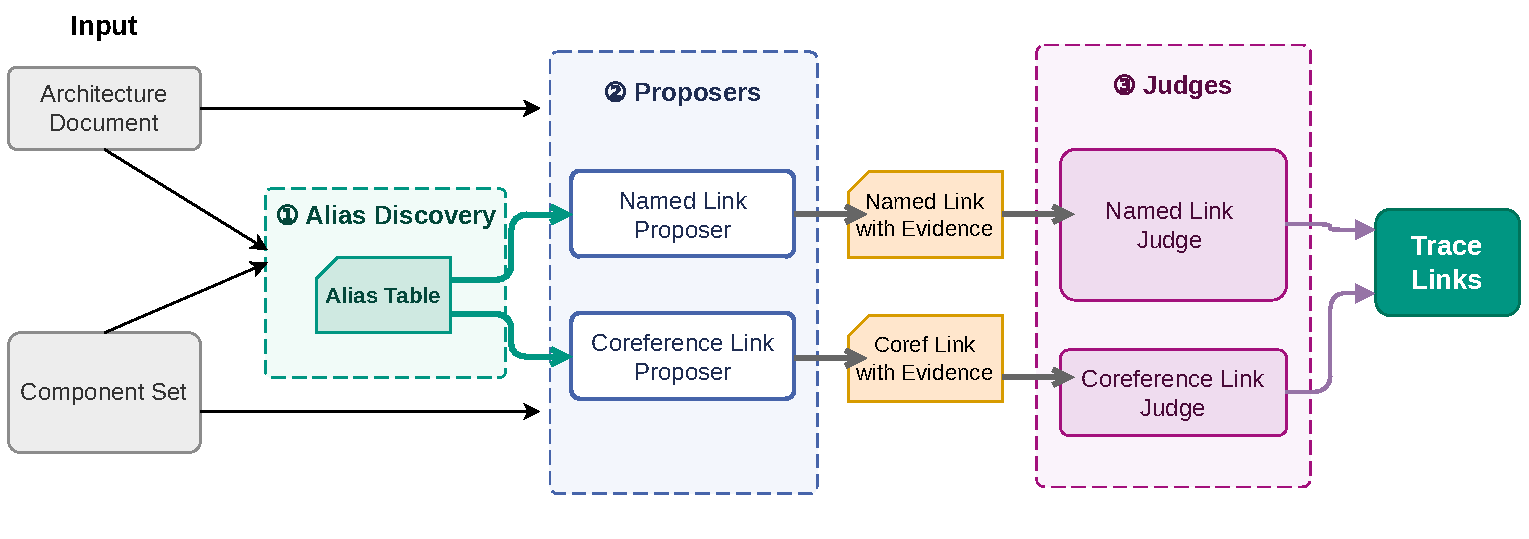
\includegraphics[width=\textwidth]{figures/approach-overview.pdf}
  \caption{Overview of \approach: a knowledge module feeds two linkers, the first
  proposing by how much of a component's name the sentence writes and the second by
  resolving a reference, each checked by its judge, then merged.}
  \Description{A workflow diagram with three stages. First, a knowledge module builds an alias table from the document and component set. Second, two linkers run in sequence: a name linker, whose two scans mark the sentences that write a whole name of a component and those that write only one word of one, and a coreference linker for sentences that write no name at all. The word scan skips any sentence that already writes a whole name. Third, each linker's candidates are filtered by its judge -- one rule for both name forms, a stricter one for resolved references -- and the surviving links are merged into the final trace-link set.}
  \label{fig:approach-overview}
\end{figure*}

\textbf{\approach in a nutshell.}
\approach answers the three challenges by three design decisions.
Targeting the challenge of various reference forms, \approach reaches them with two linker modules: the \linkerN and the \linkerC.
The \linkerN proposes candidate links by a lexical scan;
the \linkerC proposes by resolving a referring expression against the surrounding sentences.
Splitting the link recovery by form can make specialized modules do corresponding task, achieving the benefit
previous monolithic LLM call can't have.

%%%%%%%%%% C - Hallucination

To reduce the plausible but un-supported trace links, every proposed link is checked by an \ac{LLM} based judge.
Instead of merely guessing on the proposed link, we guide the judge with augmented context to reason about the architectural responsibility of the link.
Each proposer reports how the link it actually matched as a structured \emph{evidence bundle}.
The judge is prompted  with that bundle and link candidate, so this makes each judge \evidenceBacked.
This makes the result traceable to text in the document instead of to a second opinion.

%%%%%%%%%% C- Vocab
To address the vocabulary mismatch problem, \approach builds a reusable alias table.
Before linking, \approach scans the components and the document to build that table.
This is motivated by previous works on glossary mining for requirements~\cite{arora2017automated,gemkow2018automatic} and software synonym extraction~\cite{howard2013automatically,falleri2010automatic}.
Every scan and every judge reads that table, so no linker has to rediscover it mid-run.

Together these decisions give the workflow of \approach in \autoref{fig:approach-overview}: the alias discovery module, two linkers reaching three reference forms, and \evidenceBacked judges.

% -----------------------------------------------------------------
% 2.3 Knowledge discovery. The module addresses the
% ordinary-English ambiguity and the alias-discovery problem.
% -----------------------------------------------------------------
\subsection{Alias Discovery}\label{sec:doc-understanding}
Stage~1 analyzes the document against the component set to find the aliases the developers coined.
This helps linkers match a document sentence to a component even when the sentence uses a term that is not the component's exact name.
\approach discovers these aliases from the document at runtime, and they come in two kinds.
The first is an explicit renaming, where the document itself ties a short form to a name: an abbreviation or a synonym.
The second is a shorthand, one word of a multi-word name used on its own after the document has introduced the name.
An \ac{LLM} judge confirms each proposed alias before it enters the alias table, rejecting a phrase that is generic vocabulary, names the whole system, names a different component, or names a group of elements rather than one.
A term that two components both claim is taken to name neither, and is dropped before any linker reads it.
%CHECK [xx: prompt cross-ref] (filled 2026-09-07) Was: 'The prompt template is in XX.'
%  MANUAL CHECK: this is the paper's FIRST \autoref to a promptL box. main.tex defines
%  \promptautorefname and the box auto-labels as prompt:alias, but it has never been
%  compiled. Verify on the next build before trusting prompt:judge and prompt:denote too.
% The prompt template is in \autoref{prompt:alias}.

% \begin{promptL}{Alias Extraction}{alias}\\
% {\scriptsize\ttfamily\raggedright
% Find all alternative names used for these components in the document.
% COMPONENTS: \{comp\_names\}
% Find surface forms the document uses for a single named component: introduced short forms, alternate names, or one word of a\\
% multi-word name when it alone clearly means  the full name. Reject terms whose ordinary
% English use dominates. A fragment of a longer\\
% identifier is not an alias.\\
% DOCUMENT: \{doc\_lines\}\\
% Return JSON:\\
% ~~\{"abbreviations": [\{term, component\}],\\
% ~~~"synonyms": [\{term, component\}]\}
% }
% \end{promptL}

% -----------------------------------------------------------------
% 2.4 LinkerN: two scans reach the two written forms; ONE rule reads
% both, and what differs between their cases is the evidence the
% match computed. (Rewritten 2026-09-11 with the arm swap to
% s_linker120; the two separate name-linker subsections it replaces
% are in ../notes/approach-audit-trail.md.)
% -----------------------------------------------------------------
\subsection{\linkerN}\label{sec:name-linker}

% \linkerN consists of two lexical link proposers and one \ac{LLM} based judge.
% Both proposers scan the document $S$ together with the alias table, spend no \ac{LLM} call, and return candidate links, $(s,c)$ pairs.
% The \linkerB marks a sentence that writes a whole name of a component or its alias.
% The \linkerD reaches a sentence that writes only part of one: it matches a sentence word against the words of a component's name under English inflection, so a document that names an \texttt{HTML5 Client} and later writes only ``each client'' is reached where the \linkerB sees nothing.
% For example, in \autoref{fig:example} Sentence~11 writes the name of the \texttt{preferences} component, so the \linkerB proposes $(s_{11}, \texttt{preferences})$; Sentence~7 uses the same word as ordinary English while its topic is \texttt{gui}, and the proposer cannot tell the two apart, because what it knows is only that the characters are there.

Because this linking targets the simple named mention, a substring scan is enough and the proposer spends no \ac{LLM} call.
Each candidate is tagged with the matched sentence and the source, 
forming the candidate's full evidence bundle 
\texttt{\{span, naming, alias, mention\}}.
TODO XXX, explain each field.

Candidates and their evidence bundles are the input for the link judge.
In the example, Sentence~11 names \texttt{preferences} exactly, Sentence~8 writes the partial span ``model'' for \texttt{Data Model}, and Sentence~6 writes the alias ``UI'' for \texttt{gui}.
Sentence~7 uses the same word ``preferences'' while its topic is \texttt{gui}; this produces a competing name candidate even though the word is ordinary vocabulary there.
When the scanner proposes the false link $(s_{7}, \texttt{preferences})$, it is the judge's responsibility to reject it.
The judge rules once on the candidate and its bundle, weighing together whether the sentence makes an architectural claim about the component and whether the name identifies that component rather than serving as ordinary vocabulary (\autoref{prompt:judge}).
The same full bundle is used for all three written forms; only the computed field values change with the source and matched span.


% \begin{promptL}{\evidenceBacked Judge: one rule for both written forms}{judge}\\
% {\scriptsize\ttfamily\raggedright
% Validate components in a document.\\
% COMPONENTS: \{comp\_names\}\\
% A trace link holds between a sentence and a\\
% component when the sentence makes an\\
% architectural claim about that component: when\\
% it says something about that component as a\\
% participant in the system this document\\
% describes. A mention that says nothing further\\
% about the component still counts as a valid\\
% link.\\
% Every case gives you the expression, the\\
% sentence, the evidence, and, where the sentence\\
% writes a name of it, the component that name\\
% reaches. A case whose sentence writes no name\\
% of any component carries no component: decide\\
% what the expression denotes there, and nothing\\
% about identity. The evidence says what the\\
% expression is doing here; none of it is a\\
% verdict.\\
% ~~writes: what this sentence writes of the\\
% ~~name: the whole name, a short form the\\
% ~~document established, or one word of it. A\\
% ~~shorter surface leaves more readings open; it\\
% ~~does not make the reading in front of you\\
% ~~wrong.\\
% ~~alternatives: other components whose names\\
% ~~carry the same word. They are what the\\
% ~~expression could be reaching instead.\\
% ~~mention: what the code can tell about the\\
% ~~expression's place in the sentence.\\
% ~~anchors: other sentences that name this\\
% ~~component. They fix what the name means in\\
% ~~the document; they do not decide this one.\\
% Reject only on a positive ground: the sentence\\
% asserts nothing of this component, the name is\\
% doing some other job here, or the sentence\\
% denies what it would otherwise say of it.\\
% Where the case gives you a component: some\\
% sentences use an ordinary English word that\\
% coincides with a component's name. Approve only\\
% when the sentence uses that word as the name of\\
% the component. Capitalization is evidence for a\\
% name and its absence evidence against; neither\\
% settles it alone.\\
% An expression occurring only inside a longer\\
% joined or dotted identifier names a piece of\\
% that identifier, not a participant. An\\
% expression denoting what a component acts on or\\
% produces refers to that thing and not to the\\
% component.\\
% For each case, first quote the EXACT words the\\
% verdict rests on, then decide approve\\
% true/false.\\
% CASES: \{cases\}\\
% Return JSON:\\
% ~~\{"validations": [\{case, claim, approve\}]\}
% }
% \end{promptL}

% \noindent The \linkerC judge does not share this rule: its cases carry no match at all, so it is given the stricter rubric of \autoref{sec:coref-linker}, which demands a genuine referring expression and an architectural claim rather than reading an evidence bundle.

% \begin{promptL}{The reply a case with no component is asked for}{denote}\\
% {\scriptsize\ttfamily\raggedright
% (same rule and same cases as \autoref{prompt:judge};\\
% the COMPONENTS list is withheld when no case\\
% in the call carries a component)\\
% SENTENCES: \{Sn: text\}\\
% For each case, quote as the claim a contiguous\\
% exact substring of the source sentence, then\\
% answer denotation with participant or\\
% associated.\\
% Return JSON:\\
% ~~\{"validations": [\{case, claim,\\
% ~~~~denotation\}]\}
% }
% \end{promptL}

% -----------------------------------------------------------------
% 2.6 LinkerC: the shortlist is computed in code; only the reading
% of the referring expression is left to the model.
% -----------------------------------------------------------------
\subsection{\linkerC}\label{sec:coref-linker}

\linkerC recovers links where a component is mentioned by a referring expression rather than by its own name.
The coreference case may also contain an unrelated name, as Sentence~7 contains ``preferences'' while referring to \texttt{gui}; the name and coreference linkers can therefore expose different readings of the same sentence.
%CHECK [correction: no pronoun filter] (2026-09-07) The draft said 'For each sentence with
%  a pronoun like it'. s110's _resolve_references: 'Every sentence goes to the LLM in
%  context; no pronoun regex.' MANUAL CHECK: this contradicts any earlier text describing
%  a pronoun-triggered coreference stage.
A preprocessing step is annotate each sentence the exact component mentioned.
This used for the pronoun resolution. 
The resolver reads each sentence with its surrounding context and reports the referring expression, the candidate components named earlier, and the exact antecedent sentence it used.
%TODO bunblde structure. 
For illustration, Sentence~6 says ``The UI renders the main application window'', and the later Sentence~7 says ``It knows the user and their preferences.''
The resolver resolves ``It'' to \texttt{gui} through the alias-bearing antecedent in Sentence~6 and carries that exact antecedent into the judge case.
The candidates are then judged by the \corefValidator{}, which is shown the referring expression and the antecedent the resolver committed to, and rules on whether that commitment holds.

% \begin{promptL}{\linkerC: Coreference Resolution}{coref}\\
% {\scriptsize\ttfamily\raggedright
% Resolve refer-back references (pronoun or\\
% noun phrase) to components.\\
% COMPONENTS: \{comp\_names\}\\
% SENTENCES: \{Sn: text\}\\
% \{per case: TARGET Sn + NAMED BEFORE THIS\\
% ~~CASE: Name (Sm), ... nearest first\}\\
% Quote the referring expression, then the\\
% entries it could point to, then the one\\
% it does.\\
% Resolve when the surrounding sentences make\\
% one component the clear antecedent, under any\\
% form the document uses for it. Avoid\\
% resolving when two or more equally plausible\\
% antecedents exist.\\
% Return JSON:\\
% ~~\{"resolutions": [\{case, sent, ref,\\
% ~~~~candidates, component, ant\_sent,\\
% ~~~~ant\_text\}]\}
% }
% \end{promptL}
